\Chapter{Egy étterem, több futár, több kiszállítás esete}

\Section{A probléma megfoglmazása}

Jelen eset reprezentálja az egy lerakatos több ügynökös utazó ügynök problémát. Feltételek meghatározásánál nélkülözhetetlen szempont, hogy határokat szabjunk az egyes futároknak, hogy ki milyen területre szállít ki. Ennek meghatározásánál fontos a kiszállítási címek közti táv figyelembe vétele. Ezek meghatározása után maga a probléma leegyszerűsíthető egy klasszikus utazó ügynök problémára.

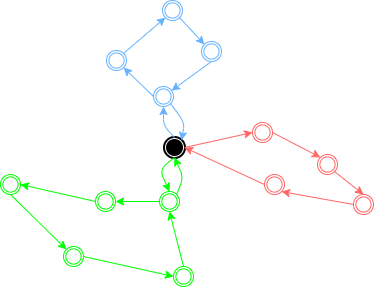
\includegraphics[scale=0.7]{images/Onedepotmtsp.png}

\Section{A probléma megoldása}

A több ügynökös, egy lerakatos utazó ügynök probléma modellje kiszállítási helyzetekre szabva\\

A több ügynökös, egy lerakatos utazó ügynök probléma esetén legyen V a csúcsok halmaza, xi,j az, hogy megy-e az i. pontból út a j. pontba közvetlenül, di,j az i. és j. pont távolsága. Legyen m az ügynökök száma és ezáltal a kapott célfüggvény:

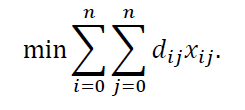
\includegraphics[scale=0.5]{images/mtsp1.png}

Minden pontba csakis egy út indul, kivétel ez alól a 0. pont ami maga az étterem:

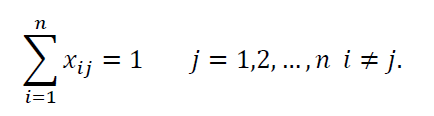
\includegraphics[scale=0.5]{images/mtsp2.png}

Minden pontból csak egy út érkezik, kivétel ez alól a 0. pont ami maga az étterem:

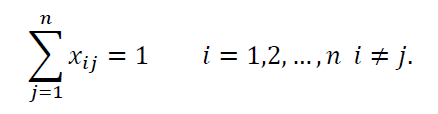
\includegraphics[scale=0.5]{images/mtsp3.png}

Az étteremre való feltétel:

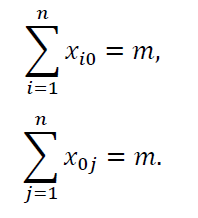
\includegraphics[scale=0.5]{images/mtsp4.png}

MTSP esetén a kövezkező megszorítások szükségessége elengedhetetlen a helyes sorrendmátrix beteljesüléséhez:

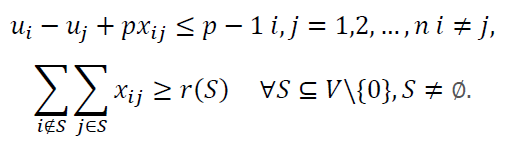
\includegraphics[scale=0.5]{images/mtsp5.png}

A definícióban S a pontok egy részhalmaza, r(S) pedig az, hogy ezt a részthalmazt minimum hány futárnak kell látogatnia. A definíció szumma része megmutatja, hogy minimum hány út megy be a vizsgált pontba. Az éttermet figyelmen kívűl hagyjuk m darab út hagyja el és m darab út megy ki belőle. Ezáltal a fenti egyenlőtlenség nem a futárok tényleges számát adná vissza. 

Magát a problémát genetikus algoritmussal oldottam meg.\\

Genetikus algoritmus \\

A genetikus algoritmusokat számítógépes szimulációkkal implementálják. A keresési tér elemei alkotják a populáció egyedeit, melyeket keresztezni (más szóval rekombinálni) és mutálni lehet, így új egyedek hozhatók létre. A keresési téren értelmezett célfüggvényt ebben a kontextusban szokásos fitness függvénynek is nevezni. A genetikus algoritmus működése során egyrészt új egyedeket hoz létre a rekombináció és a mutáció operátorokkal, másrészt kiszűri a rosszabb fitness függvény értékkel rendelkező egyedeket és eltávolítja a populációból. Egyes esetekben az ilyen algoritmusok konvergálnak az optimumhoz.

Folyamata: \\

1. Inicializáció: A kezdeti populációt legegyszerűbb véletlenszerűen generálni. A populáció mérete a probléma természetétől függ, de leggyakrabban néhány száz vagy néhány ezer egyedből áll. Hagyományosan az egyedek a keresési téren egyenletesen oszlanak el, viszont egyes esetekben olyan részeken több egyedet generálnak, ahol sejthető az optimum. \\

2. Kiválasztás: Minden sikeres generációban a jelenlegi populáció egy része kiválasztásra kerül szaporodásra. Általában fitnesz alapján történik, ahol a fittebb egyedek (a fitnesz függvény szerint) valószínűbben kerülnek kiválasztásra. Bizonyos metódusok minden egyed fitnesz-ét megnézik és választják ki a legjobbat, de más metódusok csak néhány, véletlen példányt néznek meg, mert a teljes folyamat túl hosszú lenne. A fitness függvény a példány minőségét méri. A függvény mindig probléma függő. Néhány problémánál nehéz, akár lehetetlen definiálni a fitnesz számolás műveletét; ilyenkor a példány fenotípusát is használhatjuk, vagy akár interaktív kiválasztást is használhatunk. \\

3. Szaporítás: Egyedekből újabb egyedeket a kétoperandusú keresztezés (vagy rekombináció) művelettel, és az egyoperandusú mutáció művelettel lehet. Ezeket az operátorokat általában véletlenszerűen alkalmazzák. \\

4. Leállás: A genetikus algoritmusok rendszerint addig futnak, amíg egy leállási feltétel nem teljesül. Gyakori leállási feltételek a következők: Adott generációszám elérése vagy ha a legjobb egyed fitness értéke már nem javul jelentős mértékben egy-egy iterációval.\\


\Section{A megoldás implementálása}

A programhoz tartozó fájlok\\

Dustbin\\

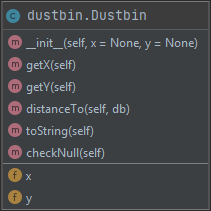
\includegraphics[scale=0.8]{images/dustbin.png}

A pontok reprezentálásához nélkülözhetetlen osztály.
\\
Galogical\\

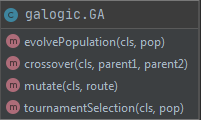
\includegraphics[scale=0.8]{images/galogic.png}

A genetikus algoritmus logikájához nélkülözhetetlen dolgokat tartalmazó osztály.
\\
Globals\\

A szimuláció futtatásához szükséges változókat, valamint a generált tartalmakat foglalja magában.
\\
Main\\

Maga a futtatható metódus.
\\
Population\\

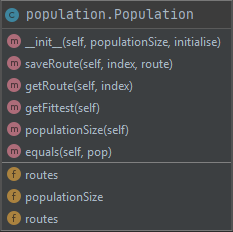
\includegraphics[scale=0.8]{images/population.png}

Az egyedeken végzett műveletekhez szükséges oszály.
\\
Route\\

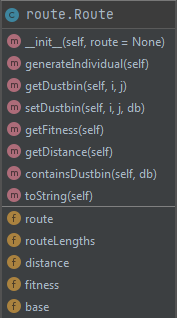
\includegraphics[scale=0.8]{images/route.png}

Az optimális út kiszámításához használt osztály.
\\
Routemanager\\

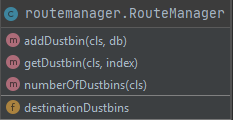
\includegraphics[scale=0.8]{images/routemanager.png}

A egyedeket kezelő osztály

\Section{A megoldás tesztelése}
